\section{TMC4671}\label{Appendix:TMC4671}

\subsection{Standard-Schaltkreis}

\begin{figure}[H]
	\centering
	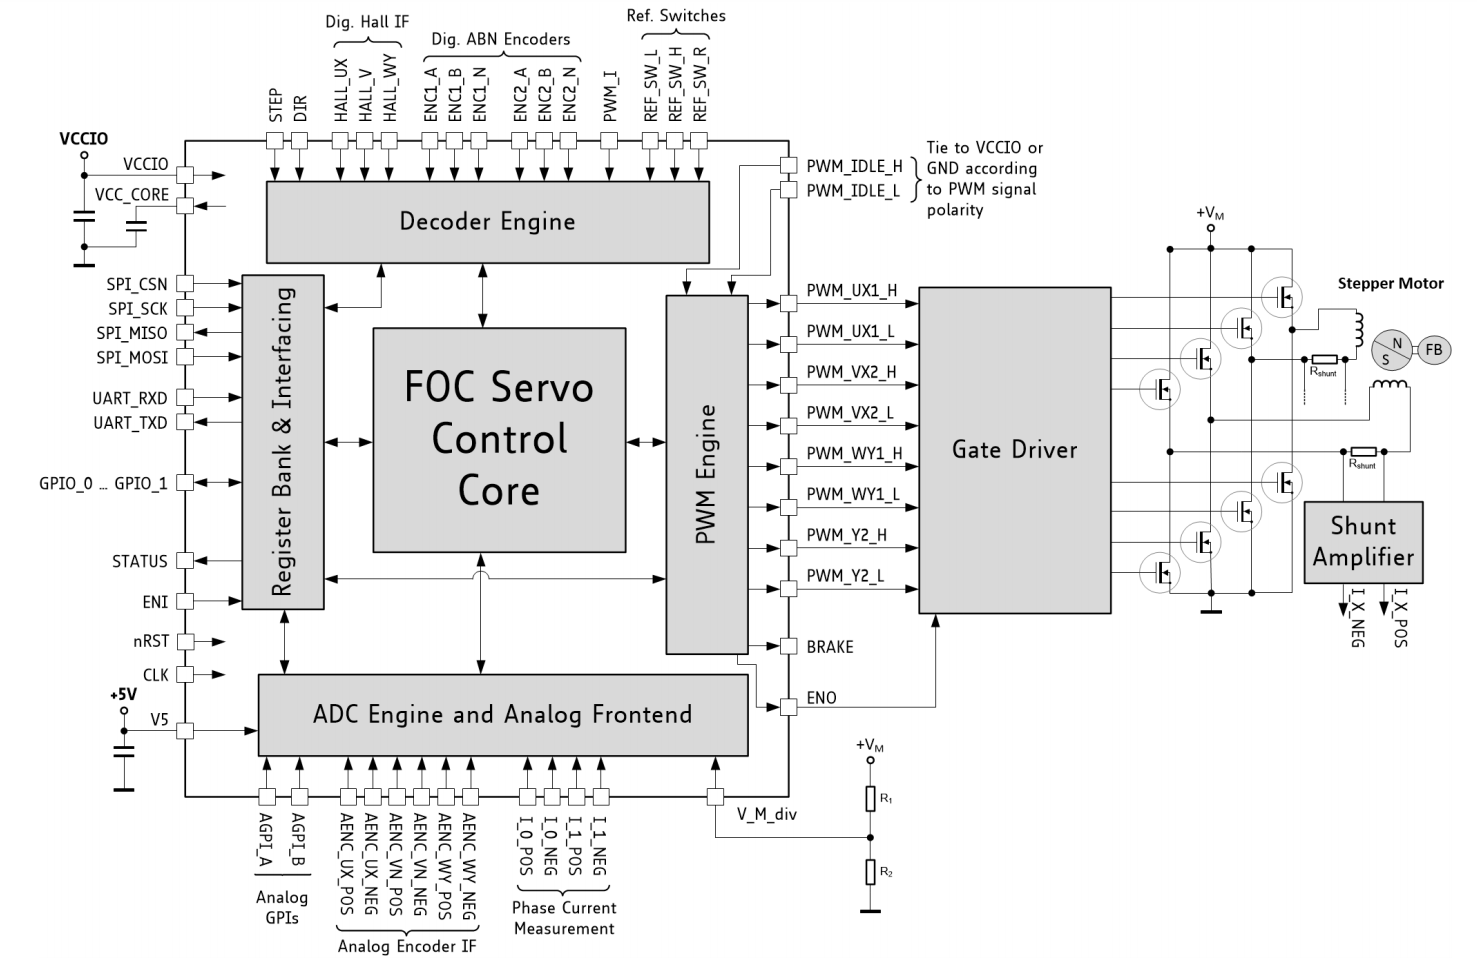
\includegraphics[width=0.8\textwidth]{graphics/Standard_Application_Cirquit_TMC4671}
	\caption{Standard-Anwendungs-Schaltung.}
	\label{fig:Schaltung_TMC4671}
\end{figure}
\todo{cite{TMC4671 Datenblatt}}

\subsection{Blockdiagramm}

\begin{figure}[H]
	\centering
	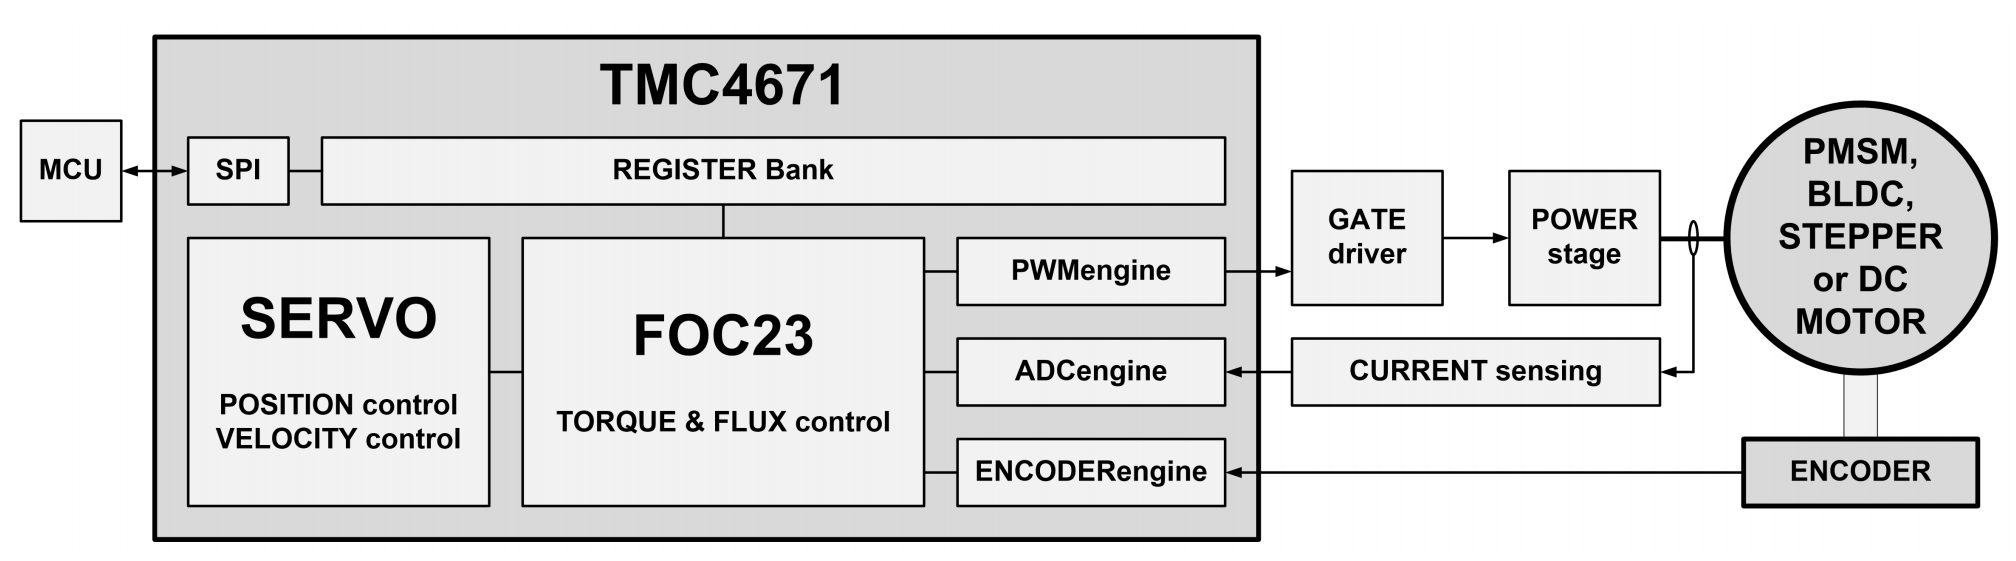
\includegraphics[width=0.8\textwidth]{graphics/Blockdiagramm_TMC4671}
	\caption{Blockdiagramm TMC4671.}
	\label{fig:Blockdiagramm_TMC4671}
\end{figure}

\todo{cite{TMC4671 Datenblatt}}

\newpage

\subsection{Inbetriebnahme}

\subsubsection{Setup}\label{Appendix:TMC4671_Setup}

\begin{figure}[H]
	\centering
	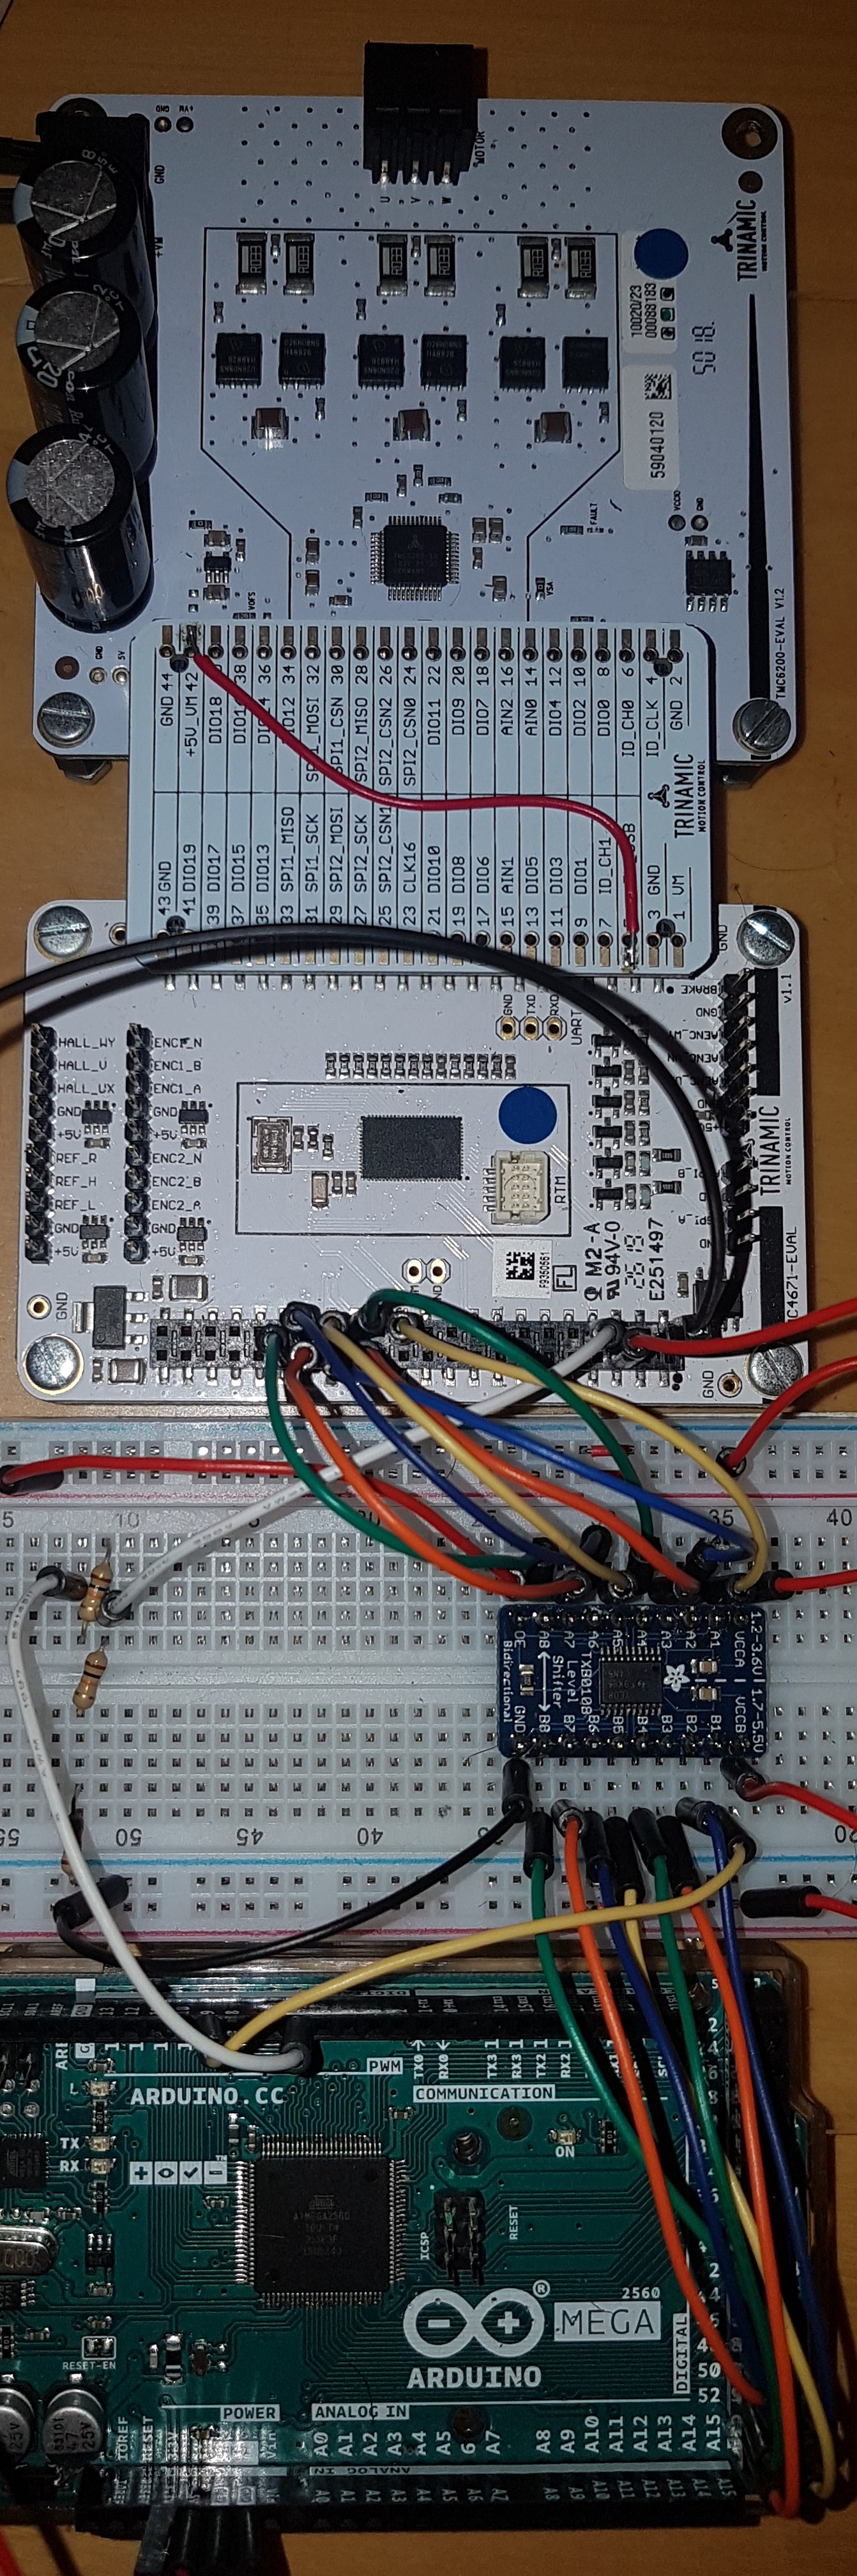
\includegraphics[angle=270,width=\textwidth]{graphics/2_komplett1}
	\caption{Gesamtansicht Setup.}
	\label{fig:2_komplett1}
\end{figure}

\begin{figure}[H]
	\centering
	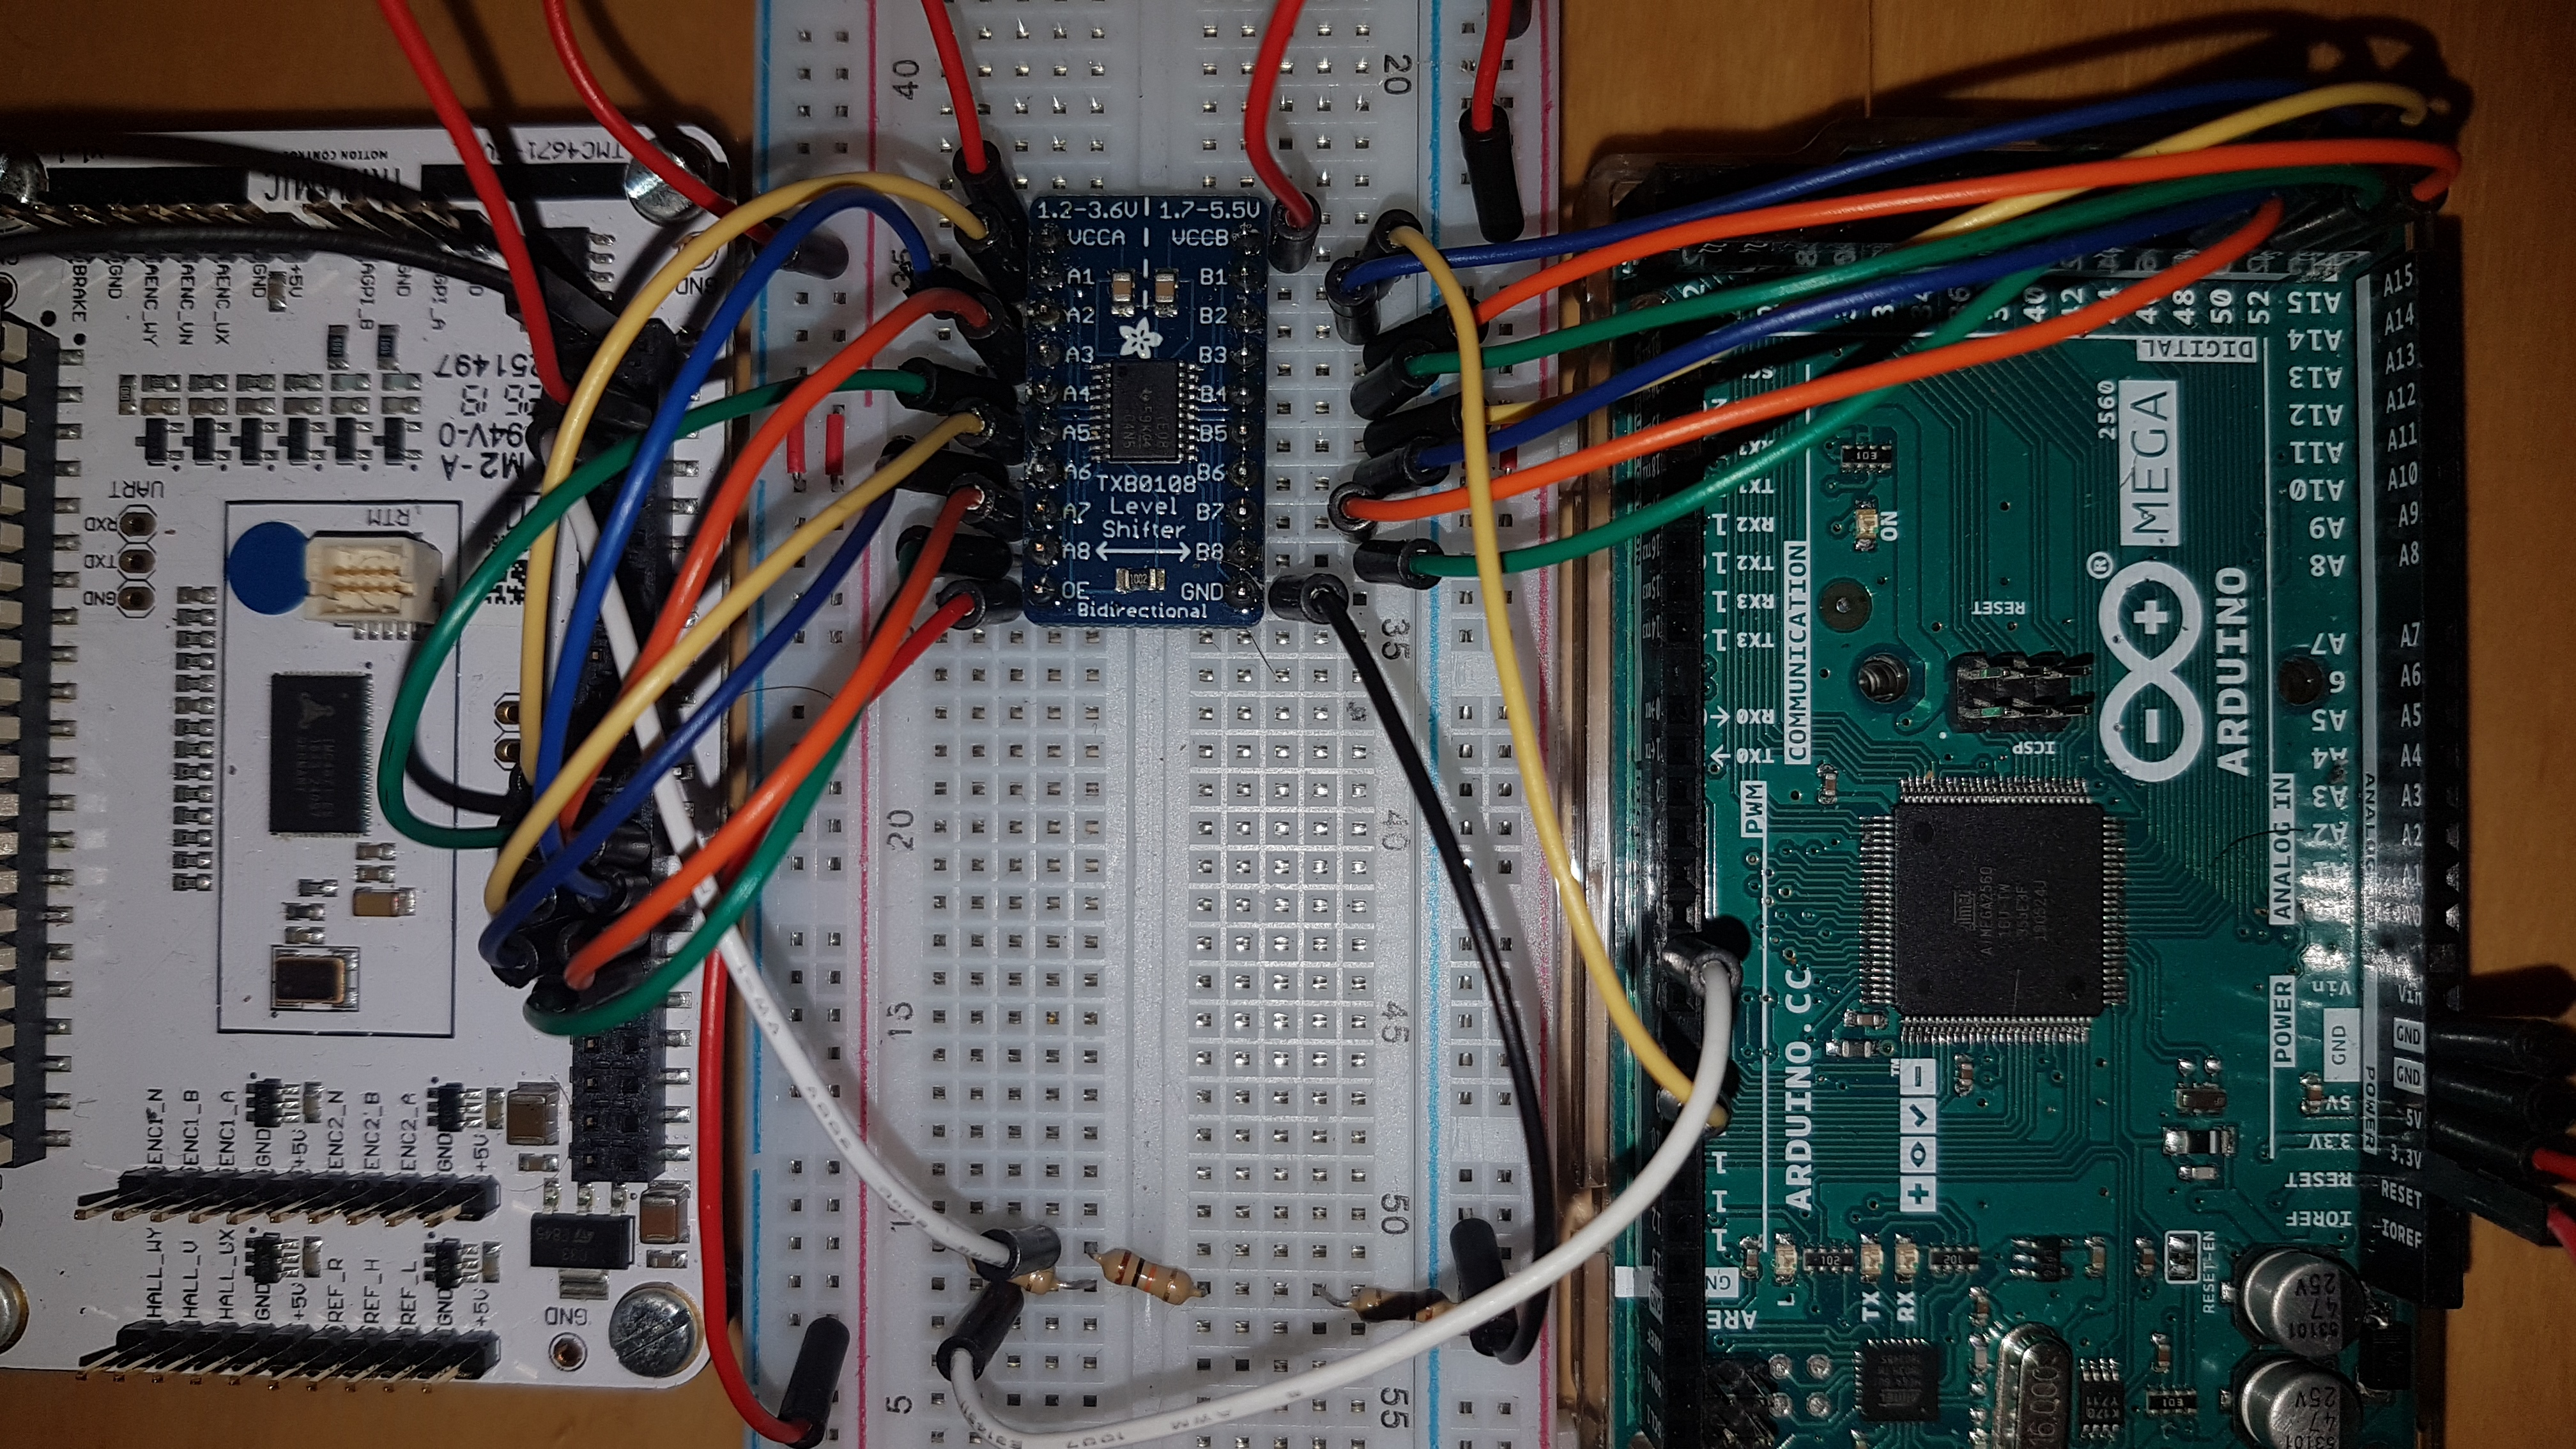
\includegraphics[angle=180,width=\textwidth]{graphics/2_komplett2}
	\caption{Gesamtansicht Setup Wiring.}
	\label{fig:1_komplett}
\end{figure}

\newpage

\begin{figure}[H]
	\centering
	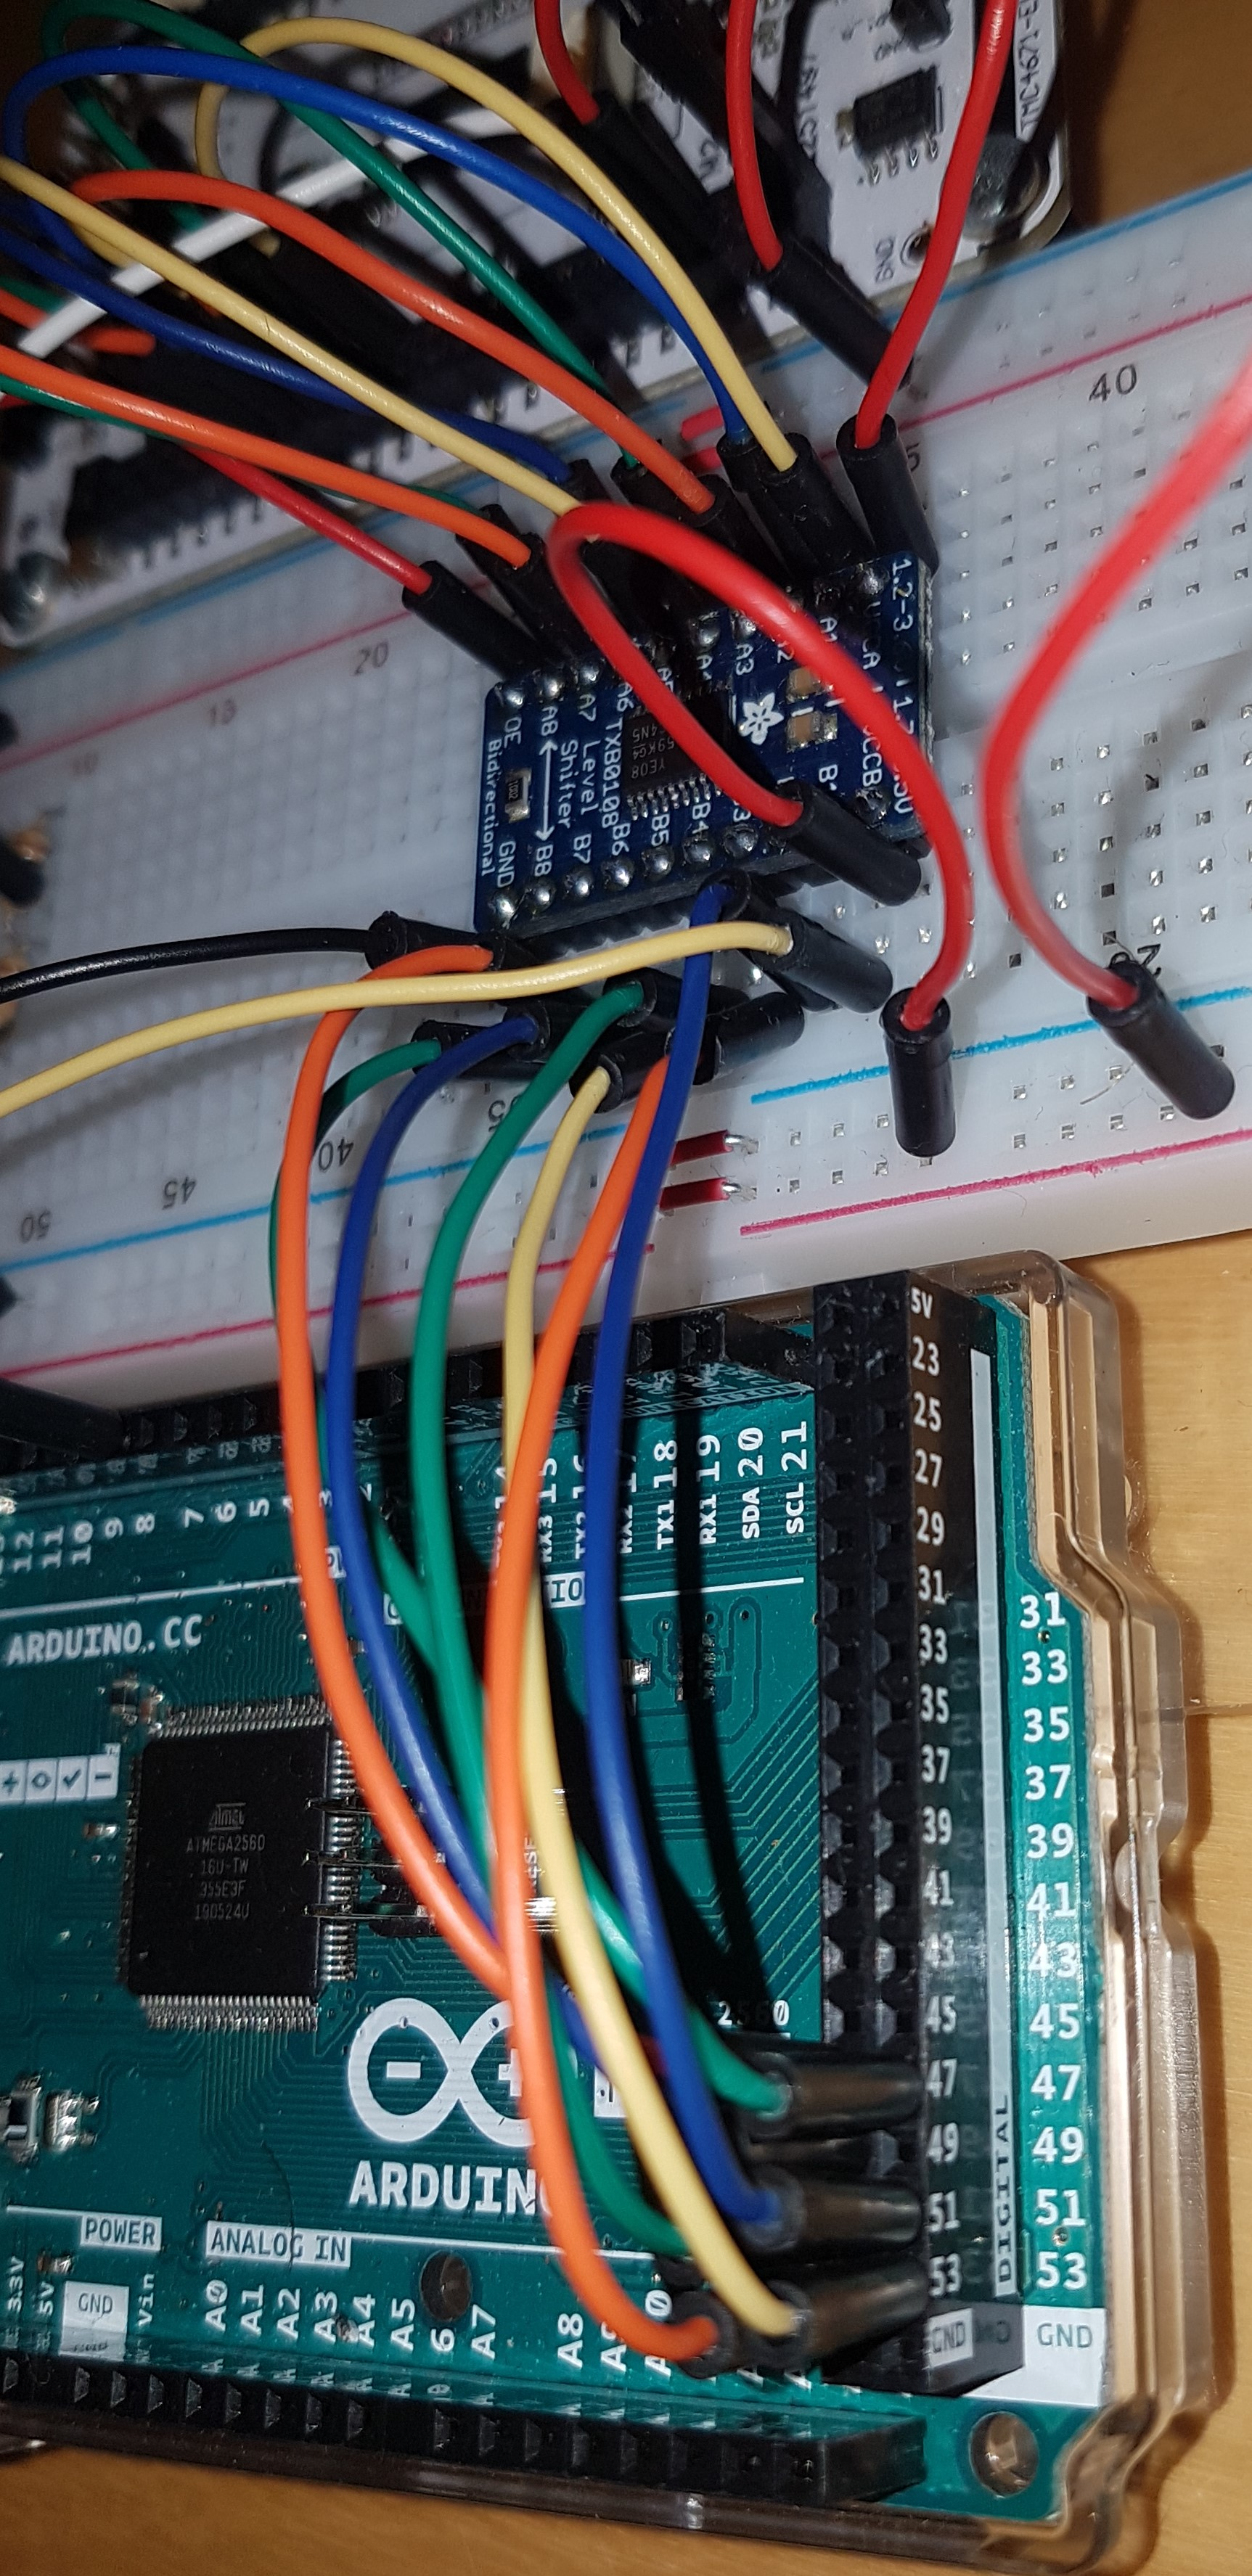
\includegraphics[angle = 270,width=\textwidth]{graphics/2_Arduino}
	\caption{Setup mit Fokus auf Arduino.}
	\label{fig:2_Arduino}
\end{figure}

\begin{figure}[H]
	\centering
	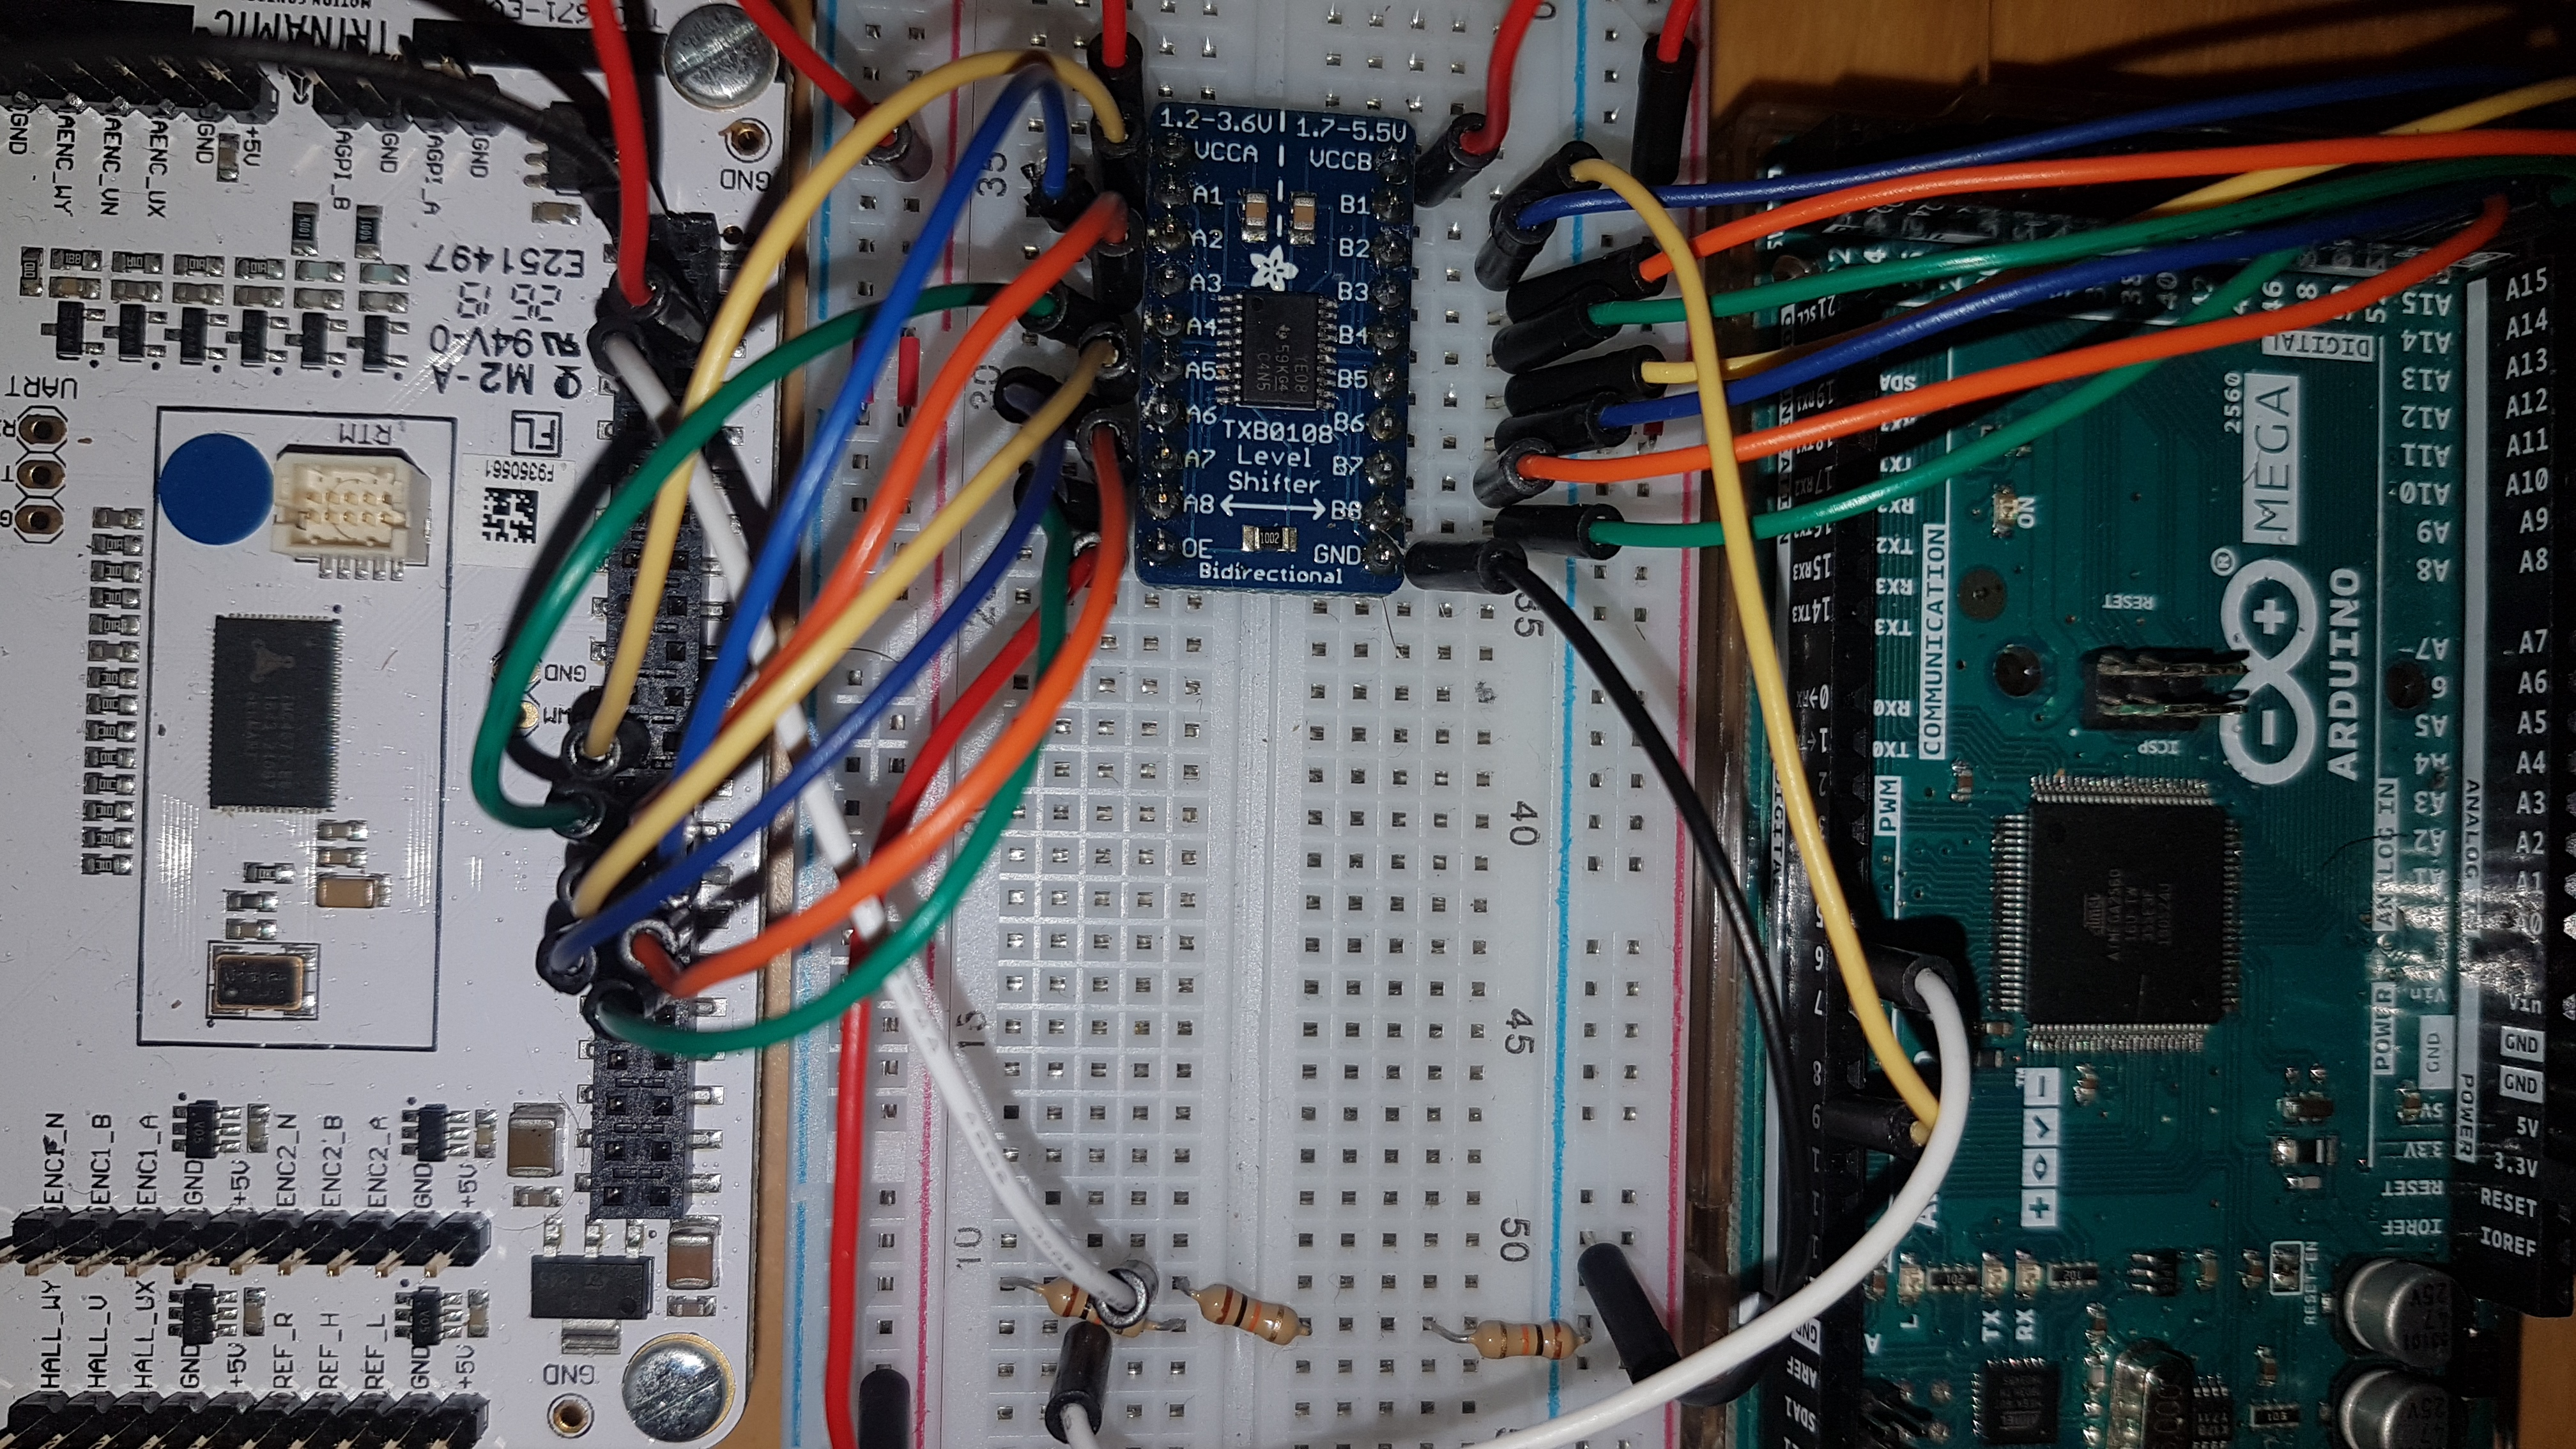
\includegraphics[angle = 180,width=\textwidth]{graphics/2_EVAL}
	\caption{Setup mit Fokus auf TMC4674-EVAL.}
	\label{fig:2_EVAL}
\end{figure}

\newpage

\subsubsection{Inbetriebnahme SPI-Kommunikation}\label{Appendix:TMC4671_SPI}

\begin{figure}[H]
\center
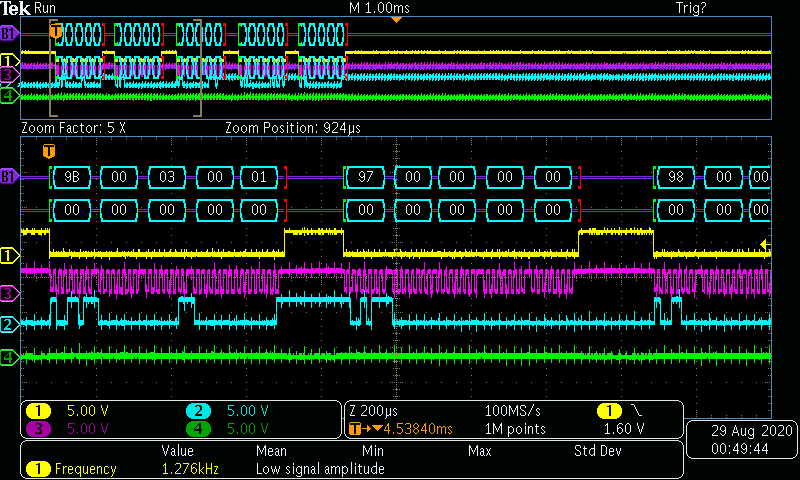
\includegraphics[width = \textwidth]{graphics/TMC4671_Beschreiben_1}
\caption{SPI-Übertragung Write (Hier Motor Pole Pairs).}
\label{fig:TMC4671_Lesen_1}
\end{figure}

\begin{figure}[H]
\center
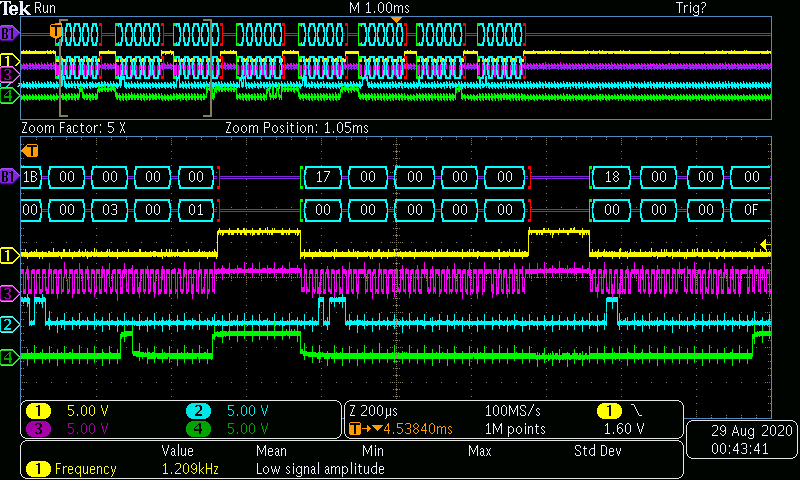
\includegraphics[width = \textwidth]{graphics/TMC4671_Lesen_1}
\caption{SPI-Übertragung Read (Hier Motor Pole Pairs).}
\label{fig:TMC4671_Lesen_1}
\end{figure}

\newpage
\begin{figure}[H]
\center
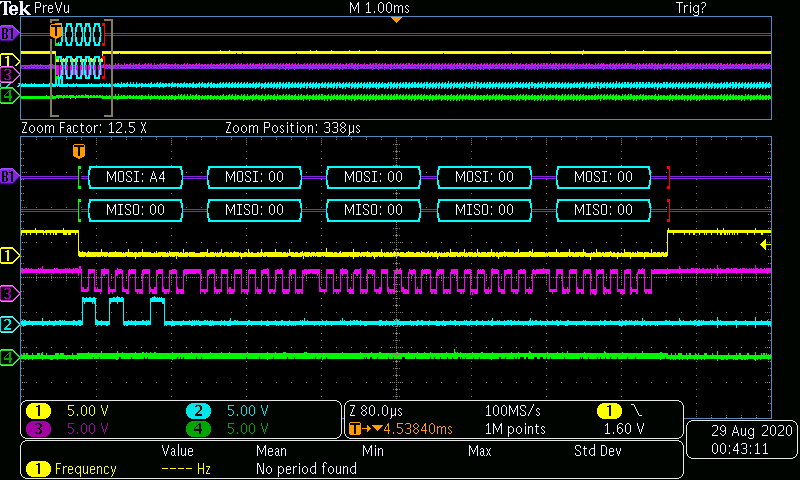
\includegraphics[width = \textwidth]{graphics/TMC4671_TestDrive4}
\caption{Übertragung mit Zoom (Testdrive).}
\label{fig:TMC4671_TestDrive4}
\end{figure}

\newpage

\begin{figure}[H]
\center
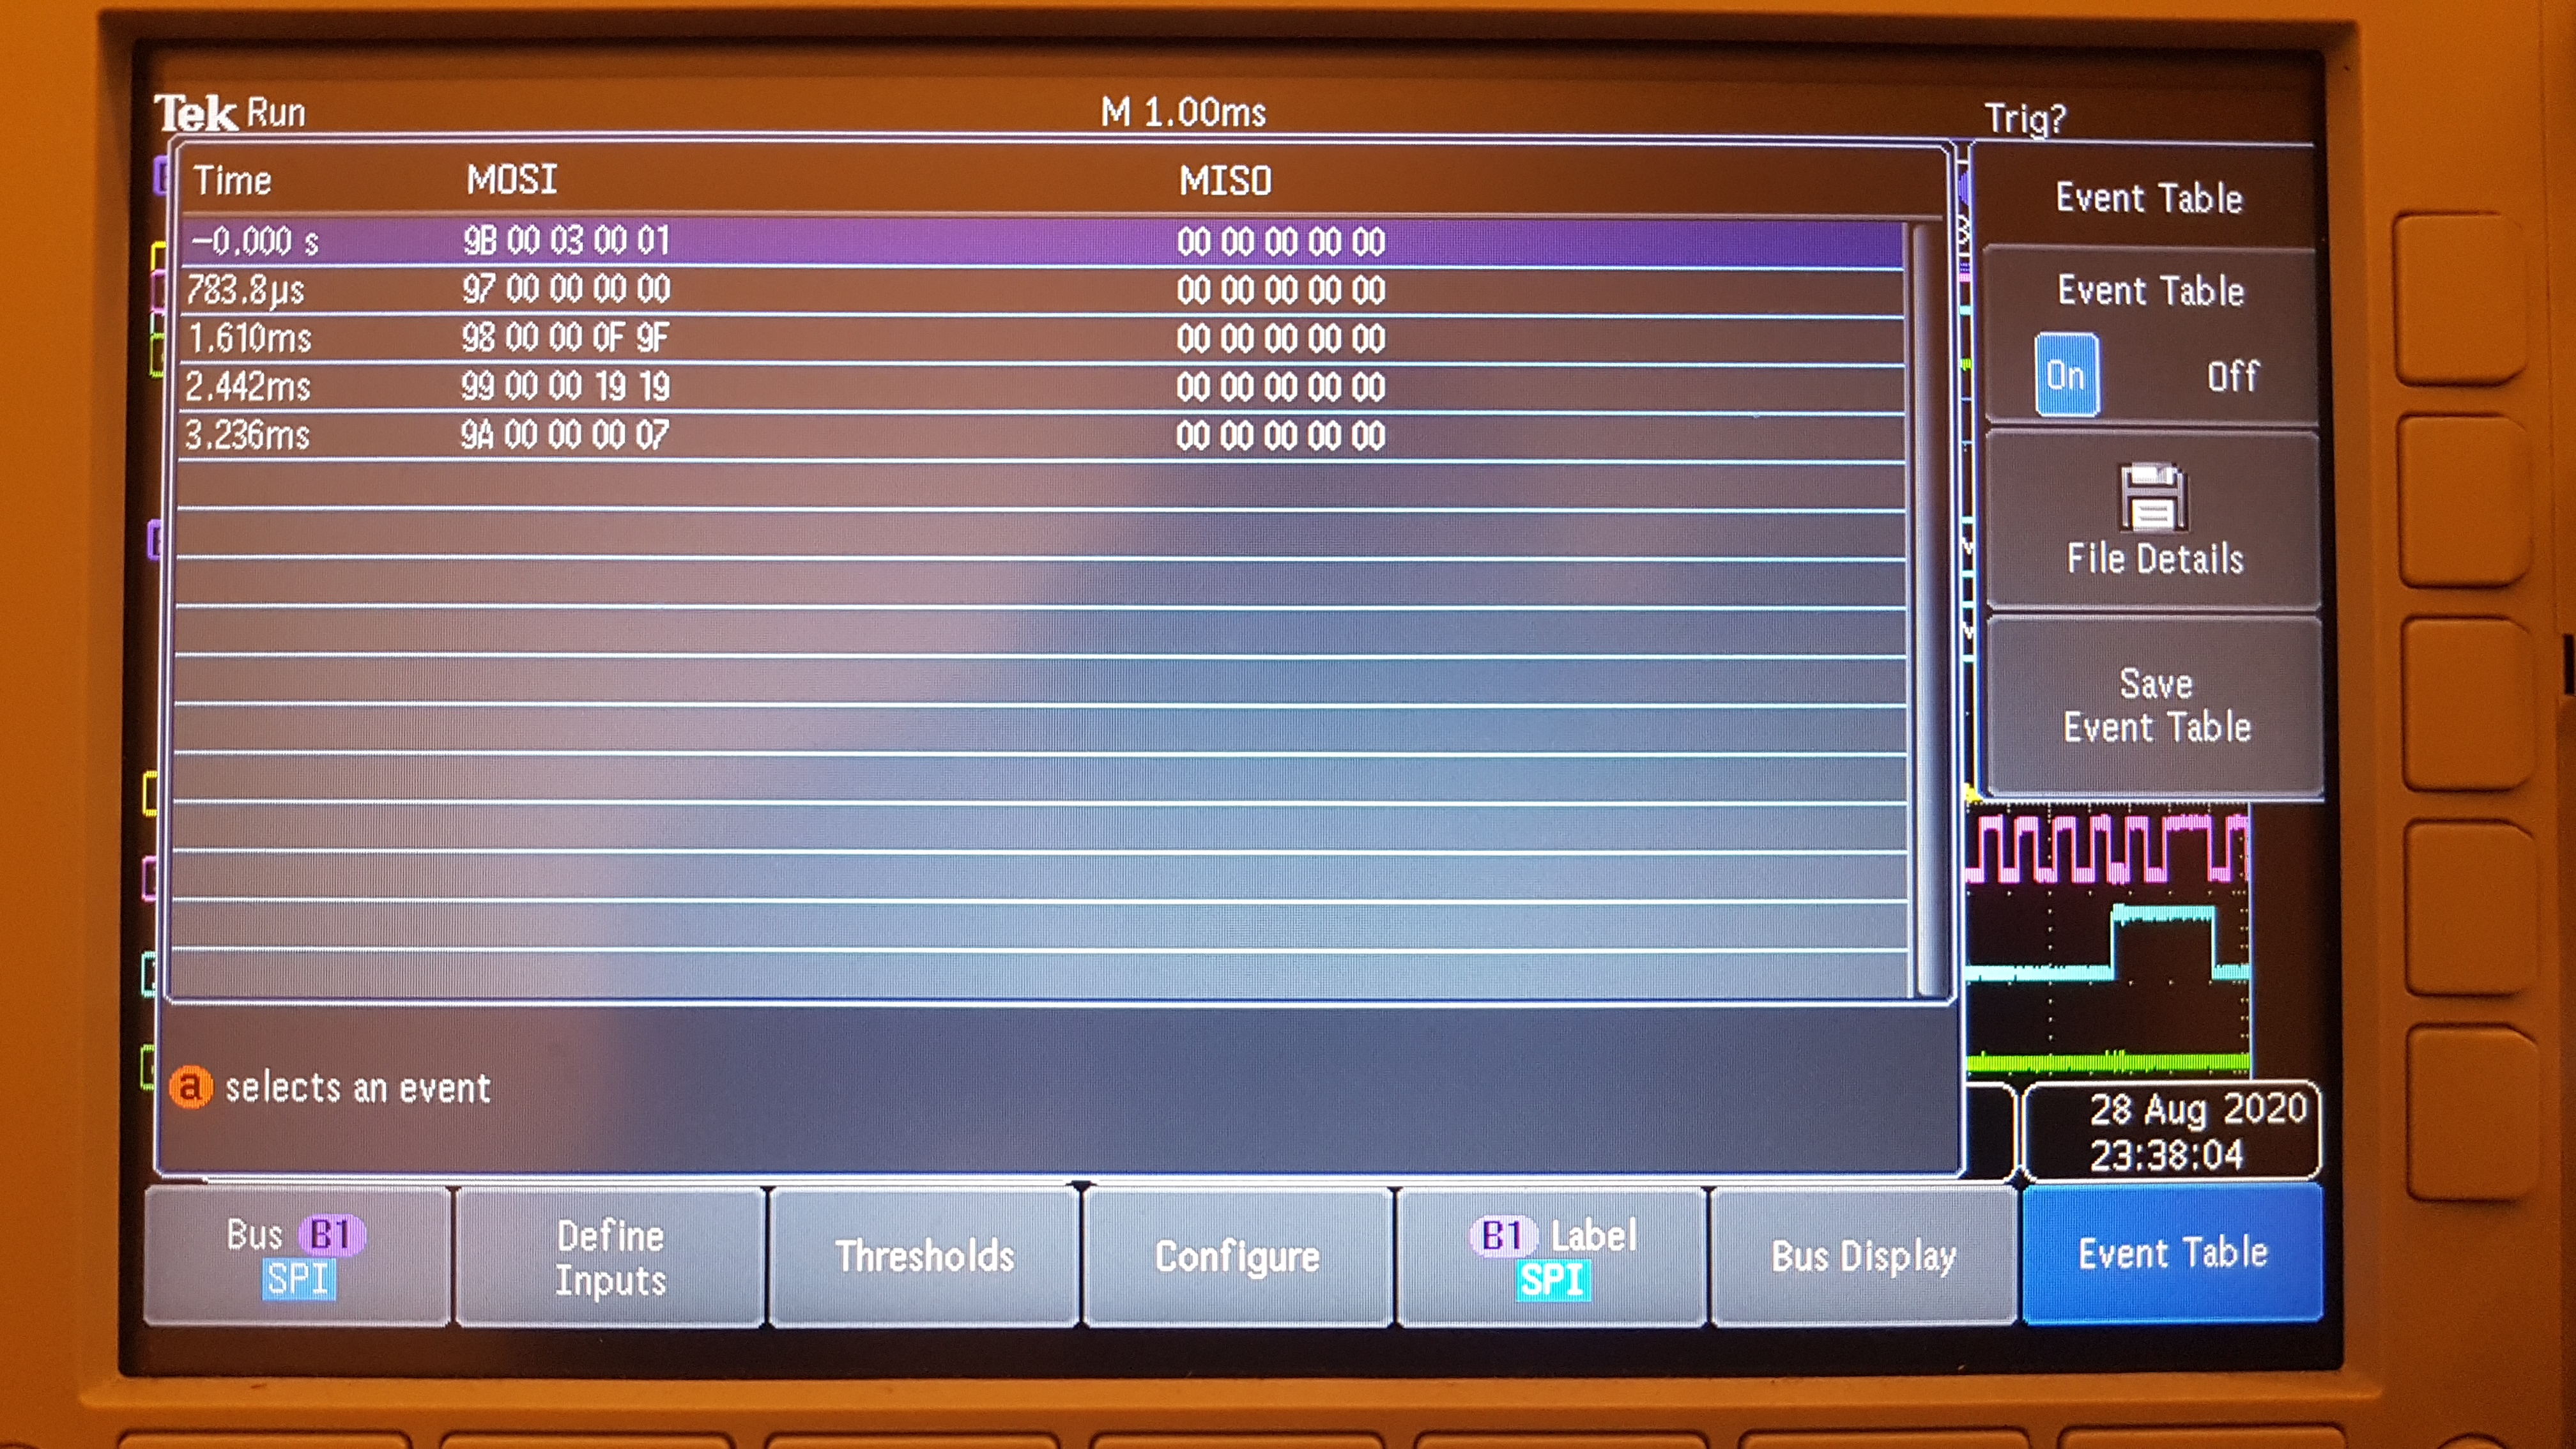
\includegraphics[width = \textwidth]{graphics/TMC4671_TimeTable_Beschreiben1_Bild}
\caption{Event-Table Inbetriebnahme TMC4671.}
\label{fig:TMC4671_TimeTable_Beschreiben1_Bild}
\end{figure}

\begin{figure}[H]
\center
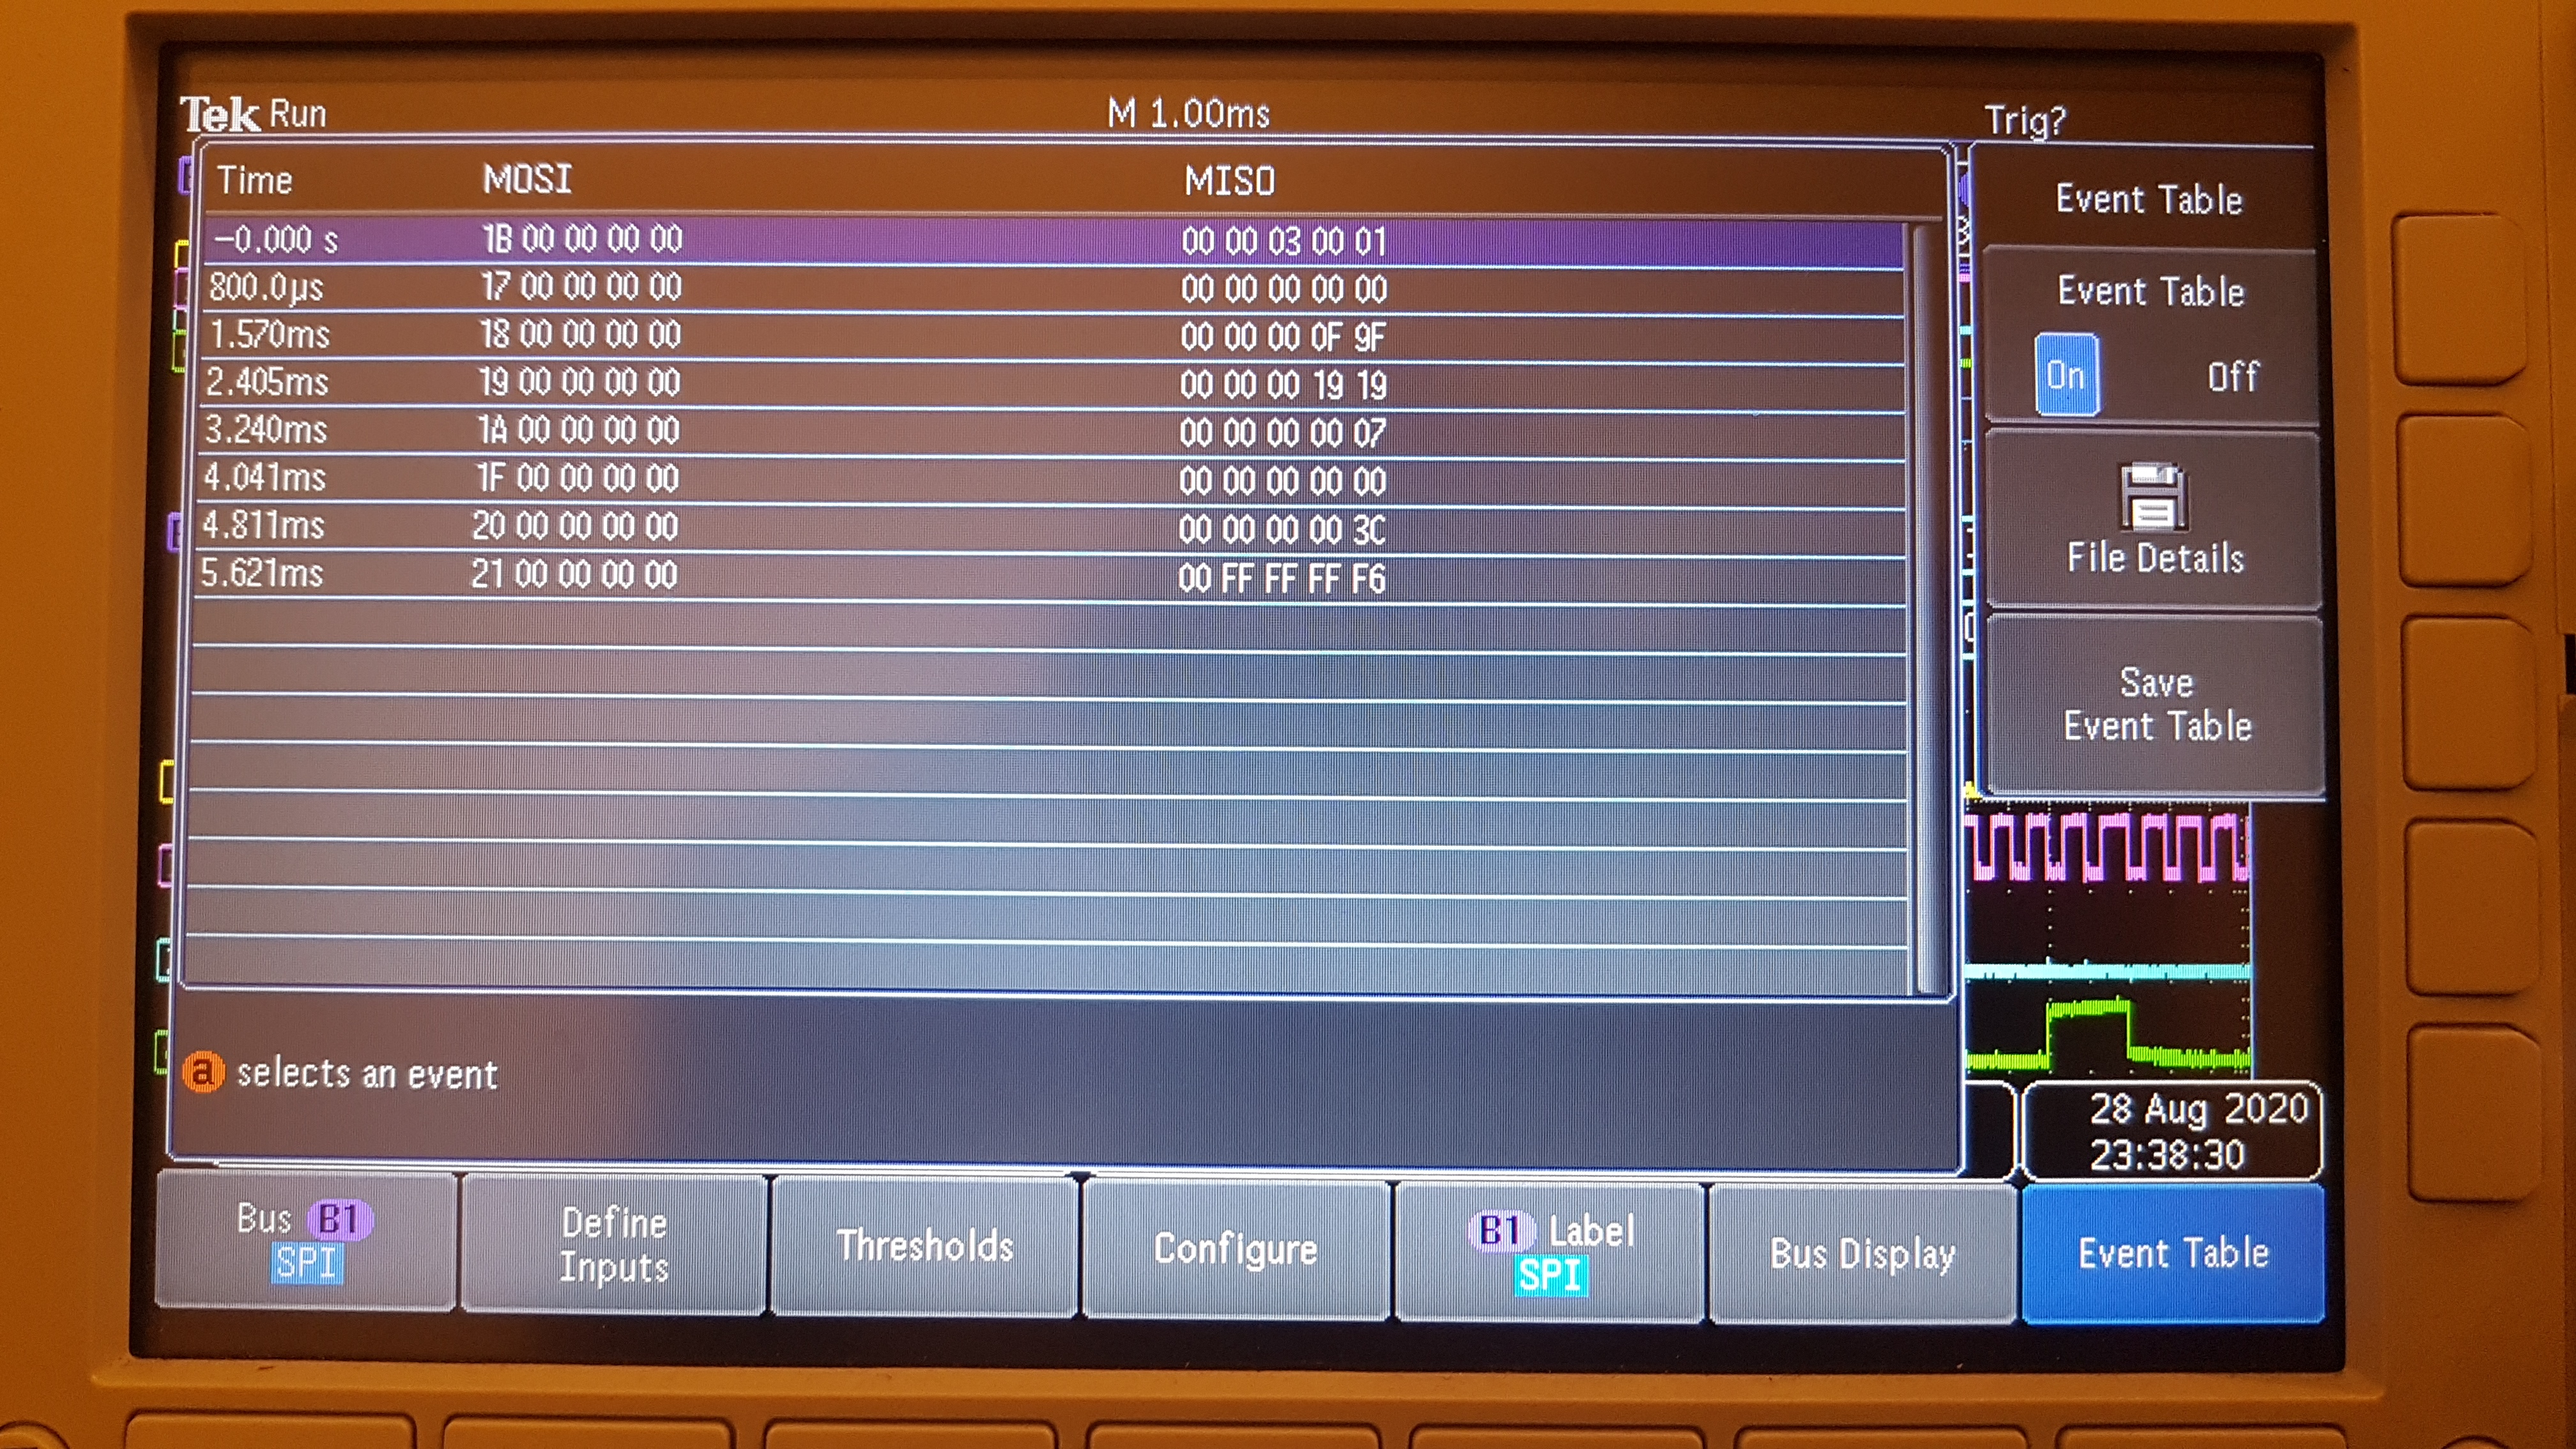
\includegraphics[width = \textwidth]{graphics/TMC4671_TimeTable_Lesen_Bild}
\caption{Event-Table Inbetriebnahme TMC4671.}
\label{fig:TMC4671_TimeTable_Lesen_Bild}
\end{figure}

\newpage

\subsubsection{Inbetriebnahme Gate-Ctrl}\label{Appendix:TMC4671_Gate_Ctrl}

\begin{figure}[H]
\center
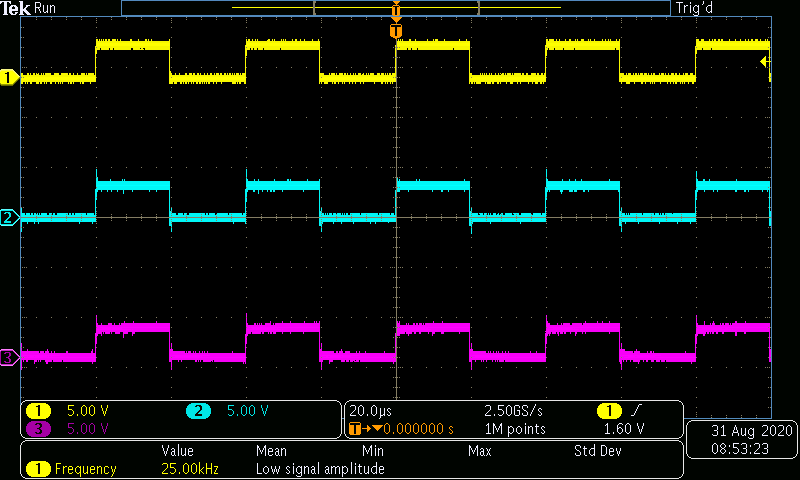
\includegraphics[width = \textwidth]{graphics/TMC4671_Gate_Signal_H}
\caption{Steuersignale PWM 48V. Gelb = U, Blau = V, Magenta = W}
\label{fig:TMC4671_Gate_Signal_H}
\end{figure}

\begin{figure}[H]
\center
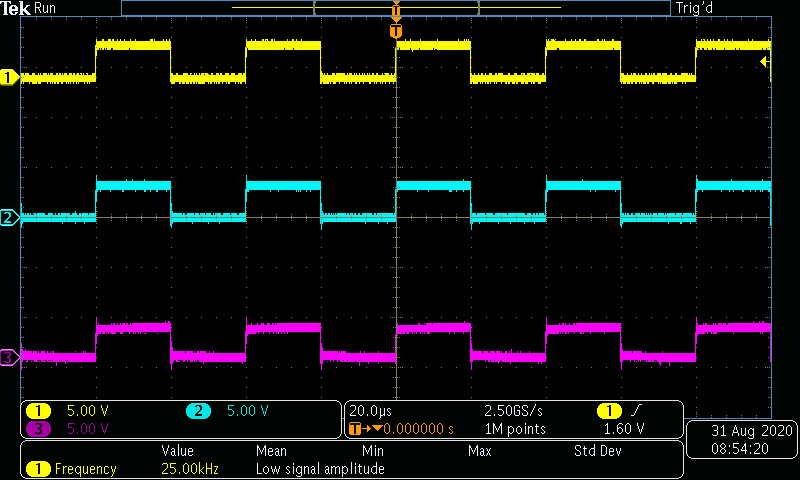
\includegraphics[width = \textwidth]{graphics/TMC4671_Gate_Signal_L}
\caption{Steuersignale PWM 0V. Gelb = U, Blau = V, Magenta = W}
\label{fig:TMC4671_Gate_Signal_L}
\end{figure}